\section{Introdução}

\begin{frame}%[allowframebreaks]
  \frametitle{Processamento de Áudio e Vídeo}
 
  \begin{itemize}
  \item Compressão
  \item Com/Sem perdas
  \item mp3, jpeg, mpeg, flac, zip, gif, png, etc
  \item sinais de áudio, fala, imagens e vídeo
  \item qualidade, taxa de compressão, custo
  \end{itemize} 

\end{frame}
\note{
  \begin{itemize}
  \item O conceito de compressão surge naturalmente quando estamos lidando com comunicação.
  \item Compressão de dados é o processo de converter dados provenientes de uma fonte em
  outros dados com menor tamanho.
  \item Armazenamento e transmissão (no fundo, ambos são formas de comunicação). 
    \begin{itemize}
    \item linha telefônica analógica
    \item comunicação digital através desta linha telefônica analógica
    \item link de comunicação de rádio entre a sonda espacial Galileu orbitando Júpiter e a Terra
    \item armazenamento e reprodução de áudio ou vídeo (ou dados) em um CD, DVD ou disco rígido
    \item reprodução celular em que a informação sobre as células é contida no DNA
    \end{itemize}
  \end{itemize}
}
\note{
  Métodos de compressão sem perda (alguns são vistos na disciplina Teoria da Informação)
  possuem como limite a entropia. Reconstrução exata da mensagem produzida pela fonte.
  Remover redundância.

  \vspace{2ex}
  Métodos de compressão com perda utilizam-se do fato de que muita informação pode ser 
  perdida sem ser percebida ou aceita-se uma distorção do sinal em prol de uma maior compressão.
}
\note{
\begin{itemize}
\item Áudio, fala, imagens e vídeo são originalmente sinais analógicos.
\item Conversão em sinais digitais: amostragem, quantização, codificação.
\end{itemize}
}
\note{
A qualidade da compressão pode ser uma medida objetiva ou subjetiva.
Na maioria das vezes, iremos realizar medidas objetivas pois realizar
testes subjetivos é muito dispendioso. Podemos escolher medidas objetivas 
que sejam bem correlacionadas com medidas subjetivas.

O custo de compressão e descompressão podem, em geral, serem diferentes.
Descompressão deve ser privilegiada pois é realizada diversas vezes e geralmente
por terminais com menor poder computacional.
}


\begin{frame}%[allowframebreaks]
  \frametitle{Imagem digital}

  \begin{figure}[h]
  \centering
  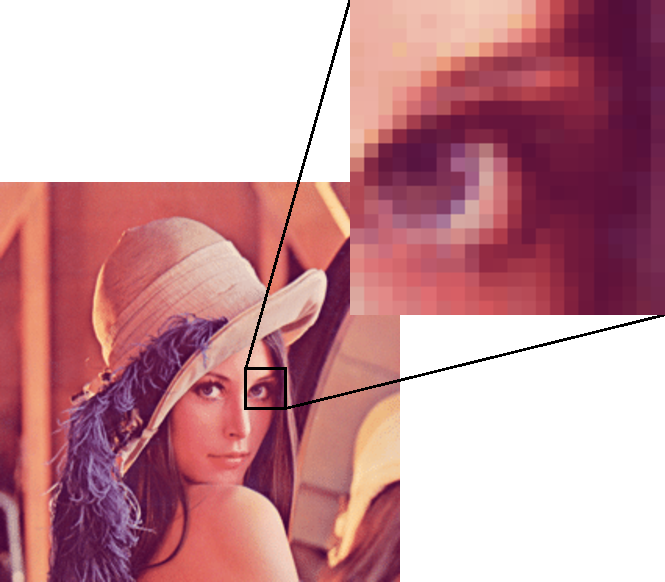
\includegraphics[width=0.5\textwidth]{images/lenaeye.pdf}
  \caption{Lena - detalhe.}\label{fig-lena-detalhe}
  \end{figure}

\end{frame} 

\begin{frame}%[allowframebreaks]
  \frametitle{Espaço necessário para armazenar uma foto}
  \begin{itemize}
  \item câmera 10 Mpixel
  \item 3 bytes por pixel (RGB)
  \item cada foto requer 30 Mbyte
  \item um cartão de memória de 2 Gbytes é capaz de armazenar 66 fotos
  \end{itemize}
\end{frame}

\begin{frame}%[allowframebreaks]
  \frametitle{Espaço necessário para armazenar um vídeo}
  \begin{itemize}
  \item 480 x 720, 30 fps
  \item 345.600 pixels por frame
  \item RGB 3 bytes por pixel
  \item 1.036.800 byte, aprox. 1 Mbyte por frame
  \item 30 frames requerem 31.104.000 bytes, aprox. 31 Mbyte por segundo
  \item um CD de 650 Mbytes é capaz de armazenar apenas 21 segundos de vídeo
  e um DVD de 4.7 GB apenas 155 segundos de vídeo.
  \end{itemize}
\end{frame}


\begin{frame}%[allowframebreaks]
  \frametitle{Dilema de compressão}
  Quando devemos parar a busca por uma \textbf{melhor} compressão?

  \vspace{1cm}
  melhor:
  \begin{itemize}
  \item menor tamanho da representação digital resultante
  \item eficiência computacional (compressão e/ou descompressão)
  \item simplicidade do algoritmo
  \end{itemize}

  \vspace{1cm}
  Qual é o limite de compressão para um determinado dado?

\end{frame} 
\note{
Modificar um algoritmo para melhorar a taxa de compressão em 1\% pode
acarretar um aumento de 10\% no tempo de execução do algoritmo e
ainda mais sobre a complexidade do programa.
}
\note{
Conjecturas\footnote{Uma conjectura é uma proposição que não é provada, mas acredita-se que seja verdadeira e não foi mostrado o contrário.}.
\vspace{2ex}

  \begin{itemize}
  \item Compressão de dados pode ser interpretada como o processo de remover complexidades (redundâncias)
  desnecessárias na informação, e desta forma, maximizando a simplicidade enquanto preserva o máximo
  possível do poder discricionário dos dados.
  \item Todo tipo de computação e racionalização formal pode ser compreendida como compressão
  de informação através do processo de identificar padrões, busca e unificação
  das instâncias destes padrões.
  \end{itemize}

}


\begin{frame}[allowframebreaks]
  \frametitle{Termos}
  \begin{description}
  \item[compressor ou codificador] é o programa que comprime os dados crus na entrada e cria uma saída de dados
  comprimida (com baixa redundância).
  \item[decompressor ou decodificador] converte os dados na direção oposta.
  \item[fluxo] é o dado a ser comprimido, armazenado como um arquivo ou transmitido.
  \item[dado não-codificado, cru, ou original] é o fluxo de dados da entrada.
  \item[dado codificado ou comprimido] é o fluxo de saída.
  \item[método de compressão não-adaptativo] é rígido e não modifica sua operação ou seus parâmetros em resposta
  aos dados em particular que estão sendo comprimidos.
  \item[método adaptativo] analisa os dados crus e modifica sua operação e/ou parâmetros de acordo com os dados em mãos.
  \item[método semi-adaptativo] utiliza 2 passagens aonde, na primeira, realiza a leitura dos dados e
  contabiliza estatísticas dos dados a serem comprimidos; na segunda passagem, realiza de fato a compressão
  utilizados parâmetros determinados na primeira varredura.
  \item[método localmente adaptativo] se adapta às condições locais do fluxo de dados e varia à medida que
  move ao longo dos dados.
  \item[compressão com perdas/sem perdas] : Para atingirem maior compressão, os métodos de compressão com perda
  perdem informação. Os métodos de compressão sem perda não admitem perder informação alguma.
  \item[Compressão em cascata] ocorre quando diferentes métodos de compressão são utilizados um em seguida do outro.
  \item[Compressçao perceptiva] ocorre quando apenas a informação imperceptível pelos nosso sentidos é removida.
  \item[Compressão simétrica] é o caso em que o compressor e descompressor utilizam basicamente o mesmo algoritmo,
  porém em direções opostas.
  \item[Complacente] é o codificador/decodificador que gera/lê de forma correta um fluxo de dados (Qualquer pessoa
  é livre para implementar seu próprio algoritmo).
  \item[Universal] é o método de compressão de dados que não depende da estatística dos dados.
  \item[Razão de Compresão] $=$ tamanho do dado de saída / tamanho do dado de entrada.
  \item[Fator de Compressão] $=$ tamanho do dado de entrada / tamanho do dado de saída $=$ (razão de compressão)$^{-1}$.
  \item[Ganho de Compressão] $= 100 \log_e $ (tamanho de referência / tamanho comprimido), aonde o tamanho de referência é o tamanho dos dados de entrada ou o tamanho do dado de saída comprimido por algum algoritmo padrão.
  \item[Erro médio quadrático (MSE) e relação sinal ruído de sinal (PSNR)] são utilizados para medir a distorção causada por uma compressão com perdas.
  \end{description}
\end{frame} 


\begin{frame}%[allowframebreaks]
  \frametitle{Termos}
  \begin{figure}[h]
  \centering
  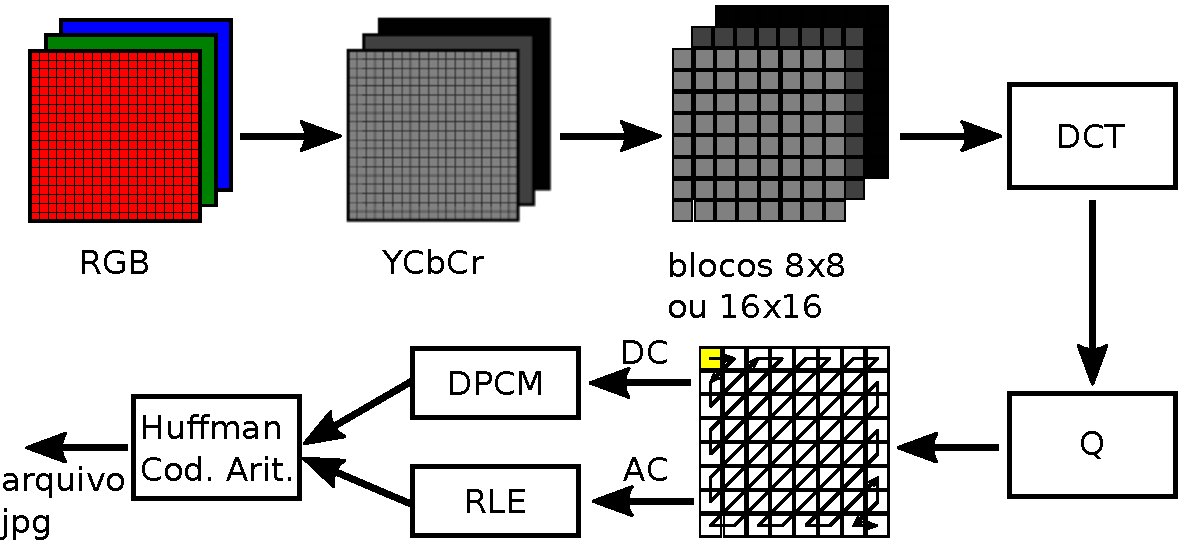
\includegraphics[width=0.8\textwidth]{images/jpegstd.pdf}
  \caption{Esquema de compressão JPEG.}\label{fig-jpegstd}
  \end{figure}
\end{frame} 

\begin{frame}%[allowframebreaks]
  \frametitle{Slides - introdução ao GNU Octave}
  \centering
  
\includegraphics[width=0.4\textwidth]{images/qrcode-octave-intro.pdf}

  \url{https://drive.google.com/open?id=1ew5fl9v_OIybsy3KdEgIvohLTcuwuru_}
\end{frame} 

\begin{frame}%[allowframebreaks]
  \frametitle{Notebook - introdução}
  \centering
  
\includegraphics[width=0.4\textwidth]{images/qrcode-jupyter-intro.pdf}

  \url{https://nbviewer.jupyter.org/github/leolca/notebooks/blob/master/aev/introducao.ipynb}
\end{frame} 

\begin{frame}%[allowframebreaks]
  \frametitle{Notebook - imagem colorida}
  \centering
  
\includegraphics[width=0.4\textwidth]{images/qrcode-jupyter-im-color.pdf}

  \url{https://nbviewer.jupyter.org/github/leolca/notebooks/blob/master/aev/introdocao_imagem_colorida.ipynb}
\end{frame} 


